\section{Implementation}

	% -介紹device跟implement細節
	% -說明real-time(列出time)

\subsection{Components}

% \begin{figure}[!t]
%   \centering
%   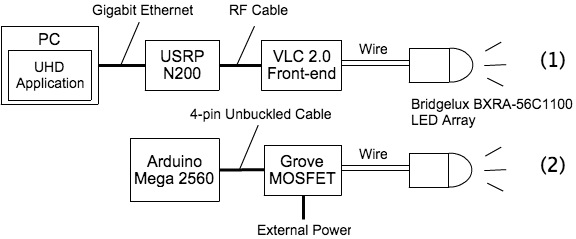
\includegraphics[scale=0.4]{pic/tx_devices.png} 
%   \caption{Transmitter Components}
%   \label{fig:tx_component}
% \end{figure}
% \begin{figure}[!t]
%   \centering
%   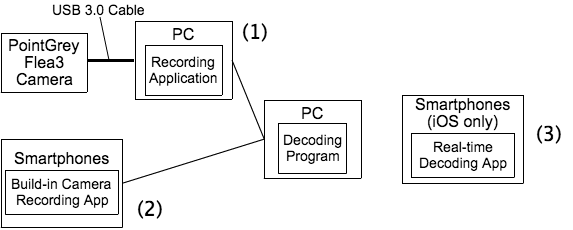
\includegraphics[scale=0.4]{pic/rx_devices.png} 
%   \caption{Receiver Components}
%   \label{fig:rx_component}
% \end{figure}

% As the system is still under development, the developed system should be sufficiently flexible so that it is easy to change various desires of the system, e.g., the modulation format, the protocol design, etc. 
% To this end, we utilize a software-defined radio (SDR) platform in our system, which enables us to make most necessary modifications in software with minimal efforts. 
% Additional hardware components were developed to interface between the SDR and the optical transmitting and receiving components. \\
% \autoref{fig:tx_component} shows the transmitter components in our proposed VLC system. 

\autoref{fig:components} shows the components in our proposed system. 
In the transmitting end, we use two different architectures to modulate the LED.
First, as the system is still under development, the developed system should be sufficiently flexible so that it is easy to change various desires of the system, e.g., the modulation format, the protocol design, etc. To this end, we use a PC with USRP Hardware Driver (UHD) application to modulate the digital information in a packet into analog signal, in the format of digitized samples. 
The software-defined radio (SDR) is connected to the PC via Gigabit Ethernet. The SDR converts the digitized samples sent from the PC into analog signal. 
The VLC 2.0 front-end board converts the voltage varying signal to current varying signal and outputs that to the LED. The signal would determine the output intensity of the LED. 

In the next stage, we try to minimize the cost of the transmitter. We use the Arduino Mega 2560 board instead, and we use Grove MOSFET which enable us to control higher voltage project, say 15VDC, with low voltage, say 5V, on microcontroller. 

In the receiving end, we just use a camera to receive the optical signal and use simple computer vision and digital image processing mechanism to demodulate. Again, we have different architectures.
First, we use PointGrey Flea3 camera~\cite{pointgrey_flea}, a high-speed camera built for experimental purposes, thus various parameters such as exposure time can be adjusted to a wide range of values. This allows us to examine system performance in different conditions. 

We also use a number of smartphones to compare their performance. We take the videos from the built-in camera app, then decoding the video on PC.

The third architecture, ideally, is to decode the preview images on the smartphone directly without storing a video and decoding at external machine. We developed an iOS app. 

% \begin{figure}[!t]
% \centering
%  \begin{subfigure}[h]{0.1\textwidth}
%   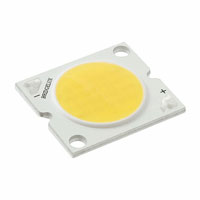
\includegraphics[width=\textwidth]{fig/LED_array.jpg} 
%   \caption{Bridgelux BXRA-W0802 LED Array} \label{fig:led_array}
%  \end{subfigure}
% ~
%  \begin{subfigure}[h]{0.1\textwidth}
%   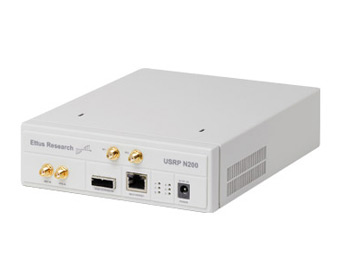
\includegraphics[width=\textwidth]{fig/usrp.jpg} 
%   \caption{USRP N200 Software Defined Radio} \label{fig:usrp}
%  \end{subfigure}
% ~
%  \begin{subfigure}[h]{0.1\textwidth}
%   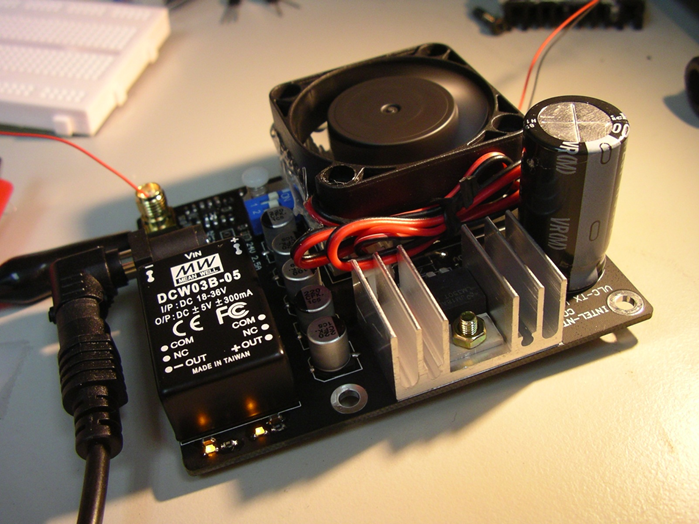
\includegraphics[width=\textwidth]{fig/VLC2_0.png} 
%   \caption{VLC 2.0 Front-end Board} \label{fig:VLC_frontend}
%  \end{subfigure}
% \caption{Photos of Transmitter Components}
% \label{fig:tx_photo}
% \end{figure}

% \begin{figure}[!t]
% \centering
%  \begin{subfigure}[h]{0.2\textwidth}
%   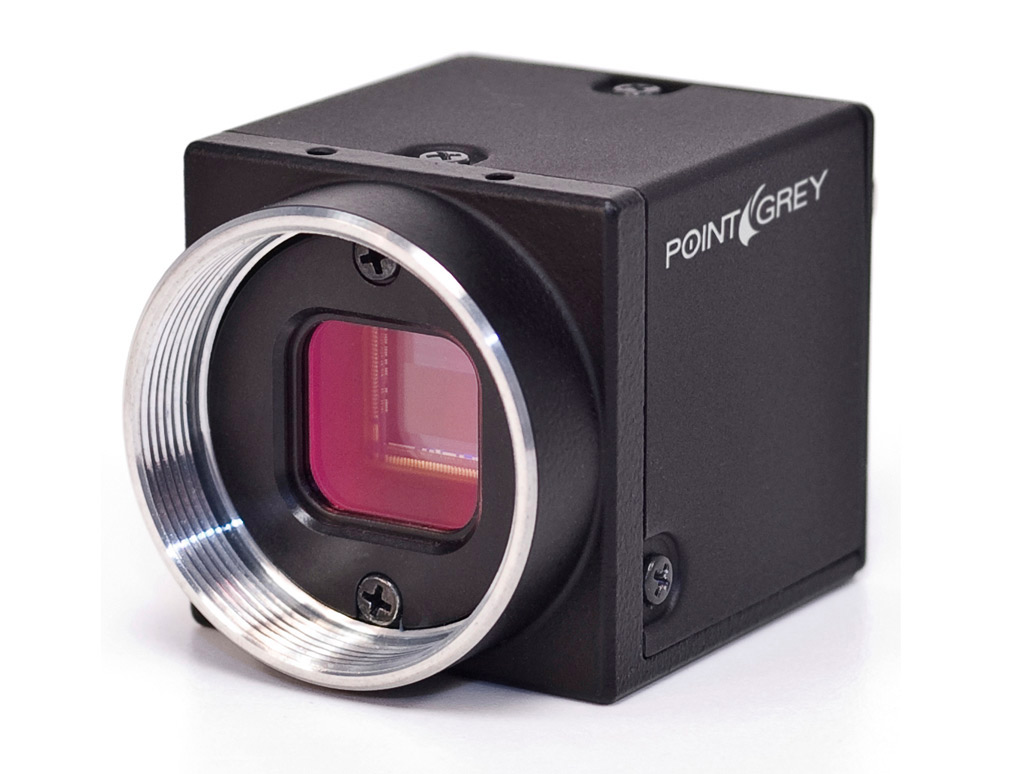
\includegraphics[width=\textwidth]{fig/flea3.jpg} 
%   \caption{PointGrey Flea3 Camera} \label{fig:flea}
%  \end{subfigure}
% ~
%  \begin{subfigure}[h]{0.2\textwidth}
%   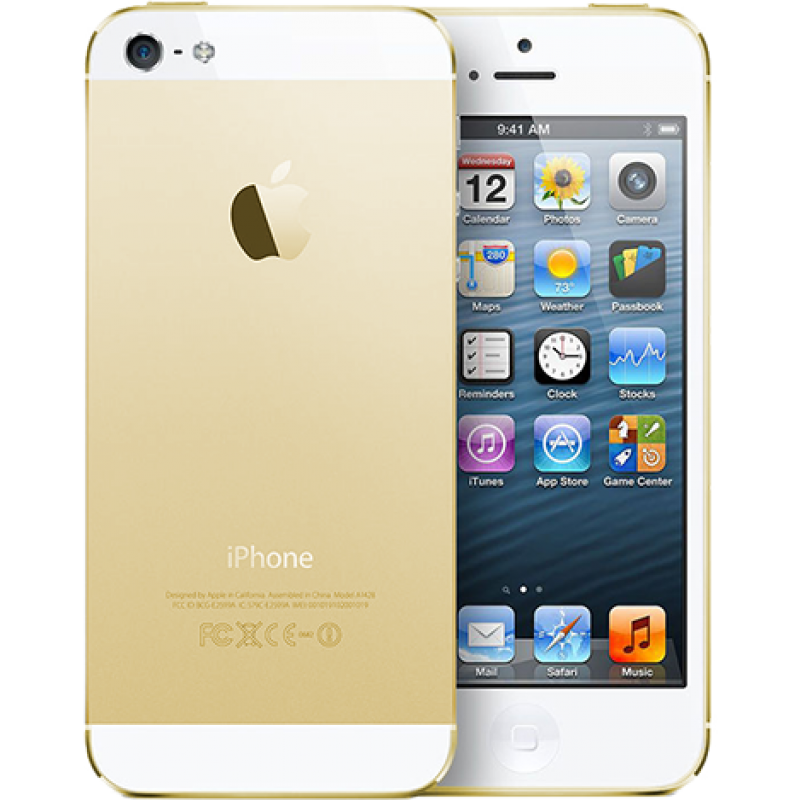
\includegraphics[width=\textwidth]{fig/iphone5s.png} 
%   \caption{SmartPhone Camera (iPhone5S)} \label{fig:iphone5s}
%  \end{subfigure}
% \caption{Photos of Receiver Components}
% \label{fig:rx_photo}
% \end{figure}

% In the following, we will describe the components in the system in detail.
% \subsubsection{LED Array}
% \autoref{fig:led_array} shows the Bridgelux BXRA-W0802~\cite{Bridgelux}, which is a high brightness LED array suitable for indoor illumination purposes and chosen as the transmitting LED component. The maximum DC forward current is 2 amps, and the typical forward voltage is around 13 volts, resulting in a maximum output power of 26 W. Typical luminous flux with 1050 mA forward is 850 lumen.

% \subsubsection{Software Defined Radio}
% As a highly flexible tool to realize the traditional RF communications, SDR has become our preferred platform to develop the VLC system. In our system, we use Ettus Universal Software Radio Peripheral (USRP) N200, as \autoref{fig:usrp} shows. USRP then converts the digital signal samples to analog voltage-varying signal.
% The unit features a gigabit ethernet interface to transfer signal samples to the PC. 
% N200 provides high-bandwidth and high-dynamic range processing capability. 
% A modular design allows the N200 to operate from DC to 6 GHz. 

% In our system we use a daughter board (LFTX) that is capable of transmitting signals from DC to 30 MHz. 
% N200 can stream up to 50 MegaSample/s to and from host applications, and users can implement custom functions in the FPGA fabric, or in the on-board 32-bit RISC softcore. The FPGA offers the potential to process up to 100 MHz of RF bandwidth in both the transmit and receive directions. 
% This is more than sufficient for our application as VLC usually operates in the range of 0.1 kHz to several kHz. The sampling rate to convert the digital samples to analog signal is configured at 1 MHz. This could emulate the clock rate of a low-cost microcontroller. Inaccuracy in the transmitted signal period could be caused by low sampling rate.

% \subsubsection{UHD}
% UHD is a driver developed by Ettus Research and is compatible with all USRP software-defined radios. 
% UHD allows development on multiple operating systems.
% UHD provides an application programming interface (API), which provides access to various functions of the USRP including synchronization, sample streaming, and configuration. 

% In the thesis, we modify one of the example applications provided with the UHD software package to modulate the transmitting signals.

% \subsubsection{VLC Front-end Board}

% The output light intensity of the LED depends on the magnitude of the input current. Thus, a hardware component is required to interface between the SDR and the LED component, linearly converting a voltage-varying signal to a current-varying signal. We utilize a custom-made VLC front-end circuit board, as shown in \autoref{fig:VLC_frontend}. 

% One of the main objectives for the design of the front-end board is to accurately convert the level of voltage in the input signal to the level of the output intensity of the attached LED. 
% For example, when the voltage of input signal is zero, the front-end would control the light intensity of the LED to be zero, and when the voltage of the input signal is raised to the maximum, the light intensity of the LED should also at its maximum. 

% Moreover, this conversion also needs to be done fast enough so that a high frequency signal can be transmitted. 

% \subsubsection{Rolling Shutter Camera}
% There are a number of cameras used in our experiments. 
%  \autoref{fig:flea} shows the specification of PointGrey Flea3 (FL3-U3-88S2C-C)~\cite{pointgrey_flea}, a high-speed camera built for experimental purposes, thus various parameters such as exposure time can be adjusted to a wide range of values. This allows us to examine system performance in different conditions. 
%  %\autoref{tab:flea_spec} lists the specification of Point Grey Flea3 camera.

% The cameras on smartphones, such as HTC New One and iPhone 5S shown in \autoref{fig:iphone5s} , are also selected for some experiments, in order to determine the expected performance of RS-FSK on cameras in off-the-shelf smartphones. 

% \begin{table}[!t]
% \centering
% \caption{Specification of Point Grey Flea3 (FL3-U3-88S2C-C).}
%   %\large
% 	\begin{tabular}{lc}
%   \hline Parameter & Value \\
%   \hline 
% 	\hline Camera Sensor Format & 1/2.5" \\
% 	\hline Type of Sensor & Sony IMX121 CMOS \\
% 	\hline Pixel (H x V) & 4096 x 2160, 2048 x 1080 \\
% 	\hline Pixel Size (H x V) & 1.55$\mu$m x 1.55 $\mu$m \\
% 	\hline Max Frame Rate (fps) & 21.6, 60 \\
% 	\hline Type of Shutter & Rolling Shutter \\
% 	\hline Exposure Time & 0.015 ms - 1 s \\
% 	\hline Estimated Read-out Time & 0.01473 ms \\
%   \hline 
% 	\end{tabular}
% 	\label{tab:flea_spec} 
% \end{table}

\subsection{Encoder} 
For the transmitting end of the system, we implement a UHD application to generate the signal. It takes a given bit stream, and produces encoded frames following a predefined bit-to-symbol mapping and the frame layout described in the previous subsection. We use 1 MHz sampling rate and a given transmitting frame rate to generate samples within one frame. These samples are then encoded with bit 1s and 0s with the corresponding symbol frequency.
The frames are then turned into analong signal and transmitted via LED light.

For another architecture, we use the Fast PWM with OCRnA top mode and the interrupt mechanism to control the clock of the Microcontroller of the Arduino Mega board. We can set the symbol frequency, the duty cycle, and the symbol duration.

\subsection{Decoder} 
We use the ffmpeg package to convert video into image frames. The decoder is implemented with OpenCV, which is a very powerful and efficient library to process images.
%The decoder is implemented in several programming languages. Two are implemented in Matlab and C++ with OpenCV for post processing and analyzing. 
The other is implemented in Objective-C with OpenCV as an iOS application for real-time processing. We will evaluate the processing time in \autoref{sec:ios_eval}.

\begin{figure}[!t]
  \centering
    \begin{subfigure}[h]{0.5\textwidth}
      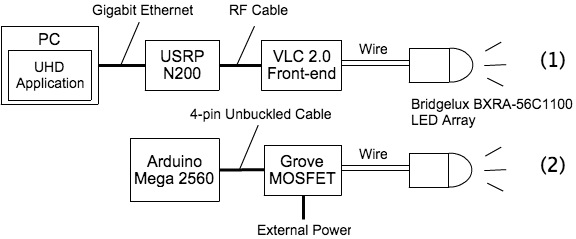
\includegraphics[width=\textwidth]{pic/tx_devices.png} 
      \caption{Transmitter Components} \label{fig:tx_component}
    \end{subfigure}
    \\
    \begin{subfigure}[h]{0.5\textwidth}
      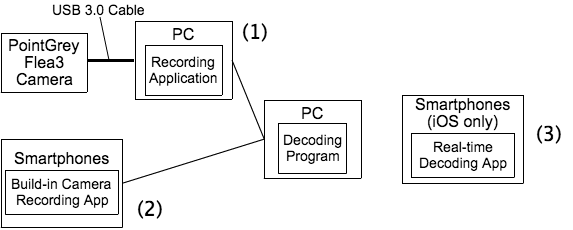
\includegraphics[width=\textwidth]{pic/rx_devices.png} 
      \caption{Receiver Components} \label{fig:rx_component}
    \end{subfigure}
  \caption{System Componenets}
  \label{fig:components}
\end{figure}